\documentclass[11pt,norsk,a4paper]{book}
\usepackage{../futhark} %I denne filen har vi alt av \usepackage osv
\usepackage{../prosess}
\begin{document}

%Forside:
	\thispagestyle{empty}   %Ingen sidetall
	\forside		%Denne setter inn forsiden.
	\clearpage		%Ny side
	
%Sammendrag og forord:
	\pagestyle{plain}	%Stil på sammendrag og forord.
	\pagenumbering{roman} 	%Sidetall på formen i, ii, osv. på sammendrag, forord og innholdsfortegnelse.

	\sammendrag{Tekst som skal stå i sammendrag}
	\forord{Arbeidet ble utført i forbindelse med emnet TMA4850 Eksperter i
Team - Matematikk innen anvendelser ved NTNU, Trondheim. Gruppearbeidet foregikk
over ett semester med gruppemøter hovedsaklig en dag i uka. Vi ønsker å takke
læringsassistentene Ida-Rene Jacobsen Forsberg og Sana Ahsan Khan for god hjelp
(og fasilitering) i forbindelse med prosessdelen av faget.}
	
	\clearpage		%Ny side

%Innholdsfortegnelse (automagisk)
	\setcounter{tocdepth}{1}
	\addtolength{\parskip}{-\baselineskip}
	\tableofcontents
	%\addtolength{\parskip}{\baselineskip}
	\clearpage		%Blank side
	\thispagestyle{empty}	%Uten sidetall

%Kapitler:
	\kapittelstil %Fikser stilen i kapitlene

	\chapter{Innledning}
\fancyhead{}
\section*{Innledning}
Denne rapporten er skrevet i sammenheng med faget TMA4850 Eksperter i Team våren
2011 av gruppa Fu\th ark. Rapporten har som mål å vise utviklingen til gruppa
og gruppas dynamikk gjennom prosjektet, og å bevisstgjøre medlemmene på
prosessene som har funnet sted langs veien.

Rapporten er delt inn i seks kapitler. \emph{Innledningen} leser du nå.
\emph{Presentasjon av gruppens medlemmer} tar nettopp for seg å presentere
gruppens medlemmer, deres faglige bakgrunn, erfaring med gruppearbeid og hvordan
resten av gruppa ser på medlemmet. \emph{Teori} tar for seg de forskjellige
teoretiske modellene for gruppearbeid og gruppedynamikk, og setter dem inn i en
relevant kontekst. Videre beskrives \emph{Oppstart og utvikling} i arbeidet med
prosjektet og prosessen, og til slutt drøftes \emph{Analyse av gruppearbeidet}
der vi peker på sammenhenger mellom teori og praksis i vår gruppe, ser på
gruppas bruk av regler og teori, og ser på hvordan dette stemmer med
virkeligheten. Det siste kapittelet presenterer vår \emph{Konklusjon}.
 %Kap. 1
	\chapter{Presentasjon av gruppens medlemmer}
\person{Åsmund}
Åsmund går i 4.klasse på studieretningen Teknisk Fysikk, med fordypning 
i matematisk fysikk. Åsmund har jobbet med numerikk og fysikk på sin forrige 
sommerjobb, og i tillegg gjør hans gode generelle kompetanse i fysikk at han 
er godt skikket til å finne de riktige differensiallikningene som beskriver
det fysiske systemet som skal studeres.

\subsection*{Innstilling til gruppearbeid}
Jeg har hatt både positive og negative erfaringer med gruppearbeid tidligere.
Jeg har merket meg at de gruppene jeg har negative erfaringer fra ofte har hatt
medlemmer som ikke har vært motiverte for arbeidsoppgaven. Dette har delvis
motivert mitt valg av MiA som landsby, da jeg tror at de som velger MiA er
innstilt på å gjøre en god jobb.

\subsection*{Gruppa om Åsmund}

Åsmund er gruppas fysiker. Han er flink til å ta initiativ og tar på seg mye.
Det er meget lett å spørre Åsmund, da han er imøtekommende, ressurssterk og
hjelpende av natur. I gruppearbeidet er han meget aktiv, men kan bli oppslukt i enkeltoppgaver og
melder seg da litt ut av gruppa. Han har en rik form for humor som favner
mye, noe som bidrar til god og avslappet stemning på gruppa. Åsmund er vårt
ordensmenneske, som har oversikt over de ulike trådene og syr de sammen til det
endelige resultatet, både hva angår prosess og prosjekt.

\person{Joakim}
Joakim studerer sivilingeniør Bygg- og miljøteknikk, med
spesialiseringen innenfor konstruksjonsteknikk og beregningsmekanikk. Fra før
har han erfaring med teamarbeid gjennom førsteklassefaget Fysisk
Miljøplanlegging, som på lik linje med EiT hadde en prosjektrapport og
prosessrapport som evalueringsform.

\subsection*{Innstilling til gruppearbeid}

Jeg liker å jobbe etter klare og veldefinerte problemer. Likevel
er jeg en stor tilhenger av en situasjonsbetinget lederstruktur, hvor gruppen
tilpasser seg underveis i arbeidet. På den måten, mener jeg, at hvert
gruppemedlem blir tildelt den rollen som faller han/hun naturlig, der og da.\\ 

Fra før har jeg hatt ett rent prosjektfag, der  gruppen var preget av
homogenitet, da samtlige var fra samme linje. Det er derfor ekstra spennende og
jobbe i en såpass heterogen gruppe, med hhv. en fysiker (Åsmund), programmerer
(Knut), numeriker (Turid), statistiker (Paul) og meg (konstruktør). Jeg har
utelukkende gode erfaringer med gruppearbeid, da jeg føler at jeg yter mer når
andre er avhengig av jobben jeg gjør, og vice versa.

%Min posisjon i gruppa er mindre selvsagt enn de resterende medlemmene. Da jeg har generell
%kunnskap om de fleste disipliner, har de inngående kunnskap i hvert sitt felt.
%Slik at jeg har tatt litt del i det meste, noe jeg liker godt. Jeg prøver derfor
%å legge til rette for et godt gruppemiljø, da jeg anser det som vel så viktig.

\subsection*{Gruppa om Joakim}
Joakim er gruppas humørspreder, og sørger for god stemning også når dagen blir
lang og gruppa er sliten. Joakims egentlige fagbakgrunn er litt på siden av
gruppas problemstilling, men han har vært veldig flink til å finne oppgaver som
han får gjort. Han har også mye kompetanse på områder som han ikke har drevet så
mye med, f.eks. numerikk og statistikk. Det at Joakim er en humørspreder gjør at 
han av og til sporer av, men dette er i all hovedsak positivt for gruppa. Selv om 
det går ut over den faglige produktiviteten der og da, har det bidratt til at 
gruppa har blitt mye bedre kjent, og sannsynligvis også til å øke produktiviteten 
på lang sikt.

\person{Turid}
Studerer ved linja industriell matematikk på NTNU, med hovedvekt på numerisk matematikk. Har tidligere gått på folkehøgskole ved linja søm og design og handball. Var med på UKA-06 som kostymedesigner for revyen.

\subsection*{Innstilling til gruppearbeid}
Jeg har tidligere jobbet en del i grupper gjennom studiet på NTNU. Disse
gruppene har imidlertid vært preget av en homogenitet i forhold til fagbakgrunn.
Det har gjort at vi angriper nye problemstillinger med en lik tankegang, og vi
mister evnen til å komme opp med mer kreative ideer til løsningsmetoder. De
forskjellene mellom gruppemedlemmer jeg har opplevd har ofte
grunnlag i ulike personligheter og kommunikasjonsstil. Da vi ikke har hatt noe
opplæring i å takle disse ulikhetene og de medhørende konfliktene, har
disse ulikhetene ofte hatt en negativ innvirkning på gruppearbeidet i form av
uløste konflikter og stagnering. Jeg har dermed sett fram til muligheten til å
lære mer om gruppeprosess og gruppedynamikk for å kunne takle slike
situasjoner annerledes i fremtiden. Jeg trives vanligvis godt i grupper, og synes
gruppearbeid kan være både fremmende og utfordrende. Jeg så derfor fram til å
jobbe i en mer heterogen gruppe, med tanke på fagbakgrunn.


%\subsection*{Turid om sin rolle i gruppa}
%
%Jeg valgte landbyen MIA utifra min interesse for numerisk matematikk. Jeg falt dermed ganske naturlig inn i ei rolle med ansvar for den numeriske berekninger i prosjektet. Når det gjaldt arbeide rundt gruppeprosessen merka jeg fort at jeg fekk en noe kontrollerende og styrende rolle. Jeg følte selv at det var ei nødvendig  rolla for å holde effektiviteten og fokuset oppe i denne delen av gruppearbeidet. Jeg føler dermed at denne rollen i noe grad var ei rolle som blei tilegna meg av gruppa. Som eneste jente på gruppe merket jeg og en større forventing til meg når det gjaldt refleksjoner over gruppearbeidet. Jeg fekk dermed ofte rollen som observatør av gruppa, både i prosjektarbeid og ulike prosess øvinger. 

\subsection*{Gruppa om Turid}
Turid er ansvarsbevisst og har tatt mye initiativ for prosessdelen. Hun er en
samlende faktor i gruppa, som kan hente oss inn når vi sporer av. Turid har vært
involvert i mange av konfliktene på gruppa, muligens fordi hun er jente,
men også fordi hun gjerne vil få igjennom viljen sin. Turid kaller en spade for
en spade, noe resten av gruppa setter pris på. Turid har vært aktiv i de aller
fleste diskusjoner, og er flink til å delegere oppgaver og å passe på at alle
har noe å gjøre.

\person{Paul}
Paul går i 4.klasse på studieretningen fysikk og matematikk, med spesialising i
statistikk. Han har erfaring med gruppearbeid fra prosjektoppgaver i statistikk, numerikk og matematisk modellering.

\subsection*{Innstilling til gruppearbeid}
Jeg liker å ha oversikt over arbeidsoppgaver og at gruppa har en framdriftsplan.
Jeg er flink til å lytte til andres meninger, og kommer på ting som jeg kan bidra med i gruppa.
Jeg er nøye med det jeg gjør, og står på når jeg har fått en konkret arbeidsoppgave.

\subsection*{Gruppa om Paul}
Paul er en stillferdig person i gruppesammenheng, men på tomannshånd er han mer
aktiv og vil presentere sin mening. Når en avgjørelse må tas i gruppa må han
involveres mer aktivt enn noen av de andre medlemmene. Paul er flink til å ta 
initiativ på det faglige, og veldig fokusert på oppgaven. Han koordinerer bra 
med de andre medlemmene i forhold til sitt fagfelt, og er et positivt bidrag til
gruppa. Hvis man gir Paul en oppgave, er man sikker på at den blir godt
gjennomført innen tidsfristen.

\person{Knut Halvor}
Knut Halvor studerer 4. året ved NTNU på linjen datateknikk. Studieretningen han 
har valgt er komplekse datasystemer. Tidligere har han hatt både gode og dårlige
erfaringer fra gruppearbeid. Det som går igjen fra gruppene han har hatt gode
erfaringer med er at medlemmene er innstilte på å gjøre en god jobb, og at de
har høye forventniger til hverandre.

\subsection*{Innstilling til gruppearbeid}
Jeg foretrekker å ha klare retningslinjer for hvilke oppgaver de forskjellige 
medlemmene har i gruppen. På denne måten kan oppgaver og løsningsmetoder diskuteres,
uten at de blir "overdiskutert". Selv om jeg foretrekker å ha ansvaret alene for mine oppgaver,
foretrekker jeg å jobbe sammen med andre, da diskusjoner rundt problemstillinger og
løsningsmetoder hjelper meg til å få organisert tankene mine.

\subsection*{Gruppa om Knut Halvor}
Knut Halvor er gruppas datamann, noe som definerer hans forhold til gruppa i
stor grad. Han er flink til å bidra med sin kompetanse i diskusjoner, og står på
sine meninger når man skal ta en avgjørelse som har å gjøre med hans fagfelt. På
mange måter er Knut Halvor den mest faglig kritiske i gruppa. Det at han hovedsaklig
jobber med programmering og er veldig selvstendig, er avgjørende for kvaliteten på 
gruppas sluttresultat, men har også gjort at det tok lengre tid før gruppa ble godt 
kjent med ham.

  %Presentasjon av gruppemedlemmer
	\chapter{Teori}
\section{Schwarz - gruppeteori}
\subsection{Effektivitet}


Flere faktorer påvirker en gruppes effektivitet; har gruppen et klart mål? Er
medlemmene enig om arbeidsmetode, og er de motiverte for den? For å forenkle
jobben som fasilitator, og/eller gi gruppemedlemmene mulighet til å påvirke
effektiviteten selv, har Schwarz utviklet en ``modell'' for hva som gjør grupper
effektive. Det er verdt å merke seg at Schwarz siterer George Box i
introduksjonen til kapittelet: ``All models are wrong; some are useful''.

Schwarz setter opp tre kriterier for effektivt gruppearbeid:

\begin{itemize}
\item[\textsc{Ytelse}] Tjenesten eller produktet gruppen leverer møter (eller overgår)
	forventningene og/eller kravene til de som skal bruke/motta/evaluere
	tjenesten.
\item[\textsc{Prosess}] Prosessene bak utførelsen av arbeidet vedlikeholder, eller
forbedrer, gruppemedlemmenes mulighet til å samarbeide på videre
arbeidsoppgaver.
\item[\textsc{Personlig}] Gruppeerfaringen skal bidra til personlig vekst og god
selvfølelse blant medlemmene.
\end{itemize}

Disse kriteriene er avhengige av hverandre, og for at en gruppe skal være
effektiv må den møte alle tre kritierer. Bryter gruppen på ett punkt vil det
påvirke de andre, for eksempel: Hvis en gruppe håndterer konflikter på en slik
måte at tilliten mellom medlemmene avtar, vil det på sikt føre til at medlemmene
holde informasjon tilbake fra resten av gruppen. Dette vil igjen føre til at
nøkkelinformasjon ikke er tilgjengelig for samtlige gruppemedlemmer, og gruppen
vil bli ineffektiv.

Videre beskrives måter en gruppe kan sikre seg effektivitet. En effektiv gruppe
håndterer konflikter i det åpne, og baserer seg på antagelsen om at hver enkelt
medlem er sterk nok til å takle negativ tilbakemelding. I tillegg er det viktig
å ikke bare løse konflikten, men også finne ut hva som forårsaket den. $\\$

Det er også viktig at man kommuniserer på en slik måte at mottaker og avsender
har samme oppfatning av hva som blir sagt. Altså må man passe på at det man sier
blir oppfattet korrekt, dette kan oppnås ved å ikke bare avsløre hva du har
funnet ut, men også \emph{hvordan} du kom til den konklusjonen. Ved å bruke
denne kommunikasjonsmetoden oppmuntres andre til å finne ``hull'' i logikk og
løsningsmetode, i tillegg til at mottaker blir tvunget til å komme med

motargumenter. Effektive grupper tester også ut sine antagelser, det vil si at
dersom et gruppemedlem sier noe svarer mottaker med å fortelle hva han/hun tror
den andre mente. Man minimerer da muligheten for misforståelser og videre
frustrasjon. $\\$

Effektive grupper må også ha klare definerte rammer for oppgaven som skal løses, 
det er også viktig at hvert gruppemedlem kjenner (og klarer å uttrykke) denne
oppgaven. Gruppen må også sørge for at hvert medlem har en klar oppfatning av
sin egen rolle i oppnåelsen av gruppeoppgaven. I samme omgang bør det sørges for
at beslutningsprosesser og hierarki i gruppen er klart definert og forstått. $\\$

En enkel, men god, måte og oppnå alle disse punktene på, er å bruke endel tid i
starten på å få til en bra samarbeidskontrakt. Der hvor tema som lederskap,
problemstilling, beslutningsmønstre, oppgavefordeling osv. kan innlemmes. Se
\cref{sec:kontrakt}. Schwarz har kokt alt dette ned til 9 grunnregler som skal sørge for
gruppeeffektivitet. Se \cref{sec:grunnregler}.
\clearpage

\subsection{Grunnregler}
\label{sec:grunnregler}
For å sikre effektivt gruppearbeid har Schwarz \cite{schwarz} etablert et sett
med grunnleggende regler (\cref{tab:grunnregler}), dette sørger for at gruppa har et enkelt og
oversiktlig oppslagsverk og vise til, for eksempel ved diskusjoner. I tillegg er
det en god pekepinn på punkter som bør være i samarbeidskontrakten.
\begin{center}
\begin{table}[ht!]
\begin{tabular}{r l}
1. & Test antagelser og slutninger \\
2. & Del \emph{all} relevant informasjon \\
3. & Bruk spesifikke eksempler og bli enig om betydning av fremmedord \\
4. & Forklar resonnement og intensjon. \\
5. & Fokuser på interesser, ikke posisjon. \\
6. & Kombiner støtte og granskning \\
7. & Utform fremgangsplaner og tilbakemeldingsmåter i plenum. \\
8. & Etabler metode for å ta opp ``ikke-tema''. \\
9. & Bruk et beslutningsmønster som sørger for nødvendig engasjement. \\
\end{tabular}
\caption{Schwarz' regler for effektive grupper}
\label{tab:grunnregler}
\end{table}
\end{center}

\section{Johnson \& Johnson}
\subsection{Gruppedynamikk}
Gruppedynamikk handler om den vitenskapelige studien av oppførsel i grupper.
Adferd i grupper, og forståelsen av den, er essensielt, da mennesker i all
hovedsak er gruppedyr, det være seg i familien, blant venner eller på jobb. Det
første som må læres er; ``hva er en gruppe?''. Spørsmålet er vanskeligere enn
man skulle tro, og Johnson \& Johnson (J\&J) \cite{jj} viser til at sosiologene
fortsatt ikke er enige om én definisjon. Likevel kan man si at en gruppe er en
samling av minimun to personer, som relaterer med hverandre ansikt til ansikt.
Samtlige individer i gruppa er også klar over at de er avhengige av de andre for
å få jobben gjort, i tillegg til at det er klart definert \emph{hvem} som er med
i gruppa. $\\$

J\&J påstår videre at en gruppes produktivitet er avhengig av fem
basiselementer:
\begin{itemize}
\item[$1.$] Positiv avhengighet blant medlemmer.
\item[$2.$] Individuell ansvarsfølelse.
\item[$3.$] Fremmende interaksjon.
\item[$4.$] Fungerende sosiale antenner.
\item[$5.$] Gode gruppeprosesser.
\end{itemize}
Hvis man i tillegg skal sørge for at gruppen er effektiv må gruppemedlemmene
\textbf{(1)} Sørge for at gruppens felles mål anvender hvert medlems
individuelle kompetanse, \textbf{(2)} forsikre at kommunikasjon mellom hverandre
er nøyaktig og forstås korrekt, \textbf{(3)} etablere lederskap og/eller
passende innflytelse, \textbf{(4)} implementere beslutningsmønstre som sørger
for at samtlige medlemmer kommer med innslag, i tillegg til at hver enkelts
resonnement og konklusjon er åpne for evaluering og analysering, \textbf{(5)}
etabler metoder for å håndtere konflikter konstruktivt.$\\$

\subsection{Å verdsette ulikheter}
Det er uunngåelig at en gruppe vil bestå av personer med ulike egenskaper. Det
være seg faglige, personlige, kulturelle, religiøse, etniske og så videre.
Det er viktig å sørge for at ulikhetene blant gruppemedlemmene kulminerer i noe
positivt, Johnson \& Johnson presenterer ulike måter man kan forsikre dette på.
Man må forsikre at det mellom gruppemedlemmene er en stor grad av positiv
avhengighet av hverandres arbeid. Gruppen må også forsøke å etablere en felles
gruppeidentitet som alle medlemmene kan samle seg bak, denne må være basert på
flertallets verdier. I oppstartsfasen er det viktig at det brukes tid på å lære
om forskjellene mellom medlemmene, et slikt enkelt grep kan kartlegge ulike
måter og ordlegge seg på (eksempelvis i ulike kulturer), som kan forhindre
miskommunikasjon og misforståelser på et senere stadium. $\\$

Det er også viktig at det etableres gode rutiner for konflikthåndtering, noe som
helt sikkert vil oppstå i heterogene grupper. Konfliktene bør håndteres slik at
gruppa får klarhet i hva som forårsaket uenigheten, og hva som ble gjort for å
løse den. Bruk også tid på at gruppemedlemmene skal bli kjent med hverandre på
et personlig nivå, på denne måten forsikrer man at diskusjonene mellom personene
i gruppa blir friere og bedre.

\section{Wheelan}
ubsection{Effective teammedlemmer}

Wheeland beskriver gruppemedlemmer's oppførsel og holdninger i effektive grupper. En viktig del ved å være en effektiv gruppemedlem består i å vurdere sin egen oppførsel og holdning og måten man kommuniserer med gruppa på. Teorien er presentert i form av retningslinjer. 

\begin{itemize}
\item[1.] Ikke skyld på andre for gruppas problemer
\item[2.] Vær engasjert når gruppa setter mål, roller og avklaring av oppgaver
\item[3.] Vær for en åpen kommunikasjonsstruktur der alle medlemmer deltar og blir hørt 
\item[4.] Ha en riktig fordeling mellom diskusjon av oppgaven og støttende kommunikasjon
\item[5.] Bruk en effektiv måte å løse oppgaver på, og en effektiv måte å ta avgjørelser
\item[6.] Lage normer som støtter produktivitet, innovasjon og frihet til å uttale seg
\item[7.] Bidra med normer som forfremmer produktivitet
\item[8.] Forfremme gruppearbeid
\end{itemize}

Punkt 1 kaller Wheeland for ''the fundamental attribution error'', fordi vi ofte tilskriver andres holdninger til personlige trekk uten å ta andre faktorer i betraktning. For eksempel kan vi skylde på sjefen for dårlige resultater uten å ta i betraktning budsjettrestriksjoner, og dårlig gruppesammarbeid. En gruppe blir ikke effektiv før alle tar ansvar for gruppa's samarbeid og produktivitet. \\

Punkt 2 dreier seg om å være klar over hva som foregår i gruppearbeidet. Hvis man ikke forstår hva som foregår, må man våge å spørre. Å stille spørsmål til hele gruppa vil føre til en rikere diskusjon og vil klargjøre ting for alle gruppemedlemmer. \\

Punkt 3 tar opp problemet med at medlemmer i gruppa ikke tør å si det de mener fordi de ofte klassifiserer andre i gruppa, og ut i fra det angir dem høyere eller lavere status. Disse medlemmene kan bli ignonert i gruppa, noe som fører til at gruppa blir mindre produktiv. En måte å sikre at alle blir hørt på er så enkelt som å ta en runde rundt bordet for å høre hva hver og en har å si. \\

Punkt 4 handler om oppgaveorientert diskusjon i gruppen. Forskning tyder på at suksessfulle grupper bruker om lag 70-80 \% av tiden sin til å diskutere oppgave og mål. Men ofte hender det at gruppa går seg bort i en lang diskusjon om noe annet. \\

Punkt 5 diskuterer effektive måter for oppgaveløsning og det å ta beslutninger. Det nevnes fire steg som kan følges: Å innse problemet, diagnotisere problemet, ta beslutningen, og akseptere og gjennomføre beslutningen. I praksis består de to første stegene i å planlegge strategier for å løse problemet. Når man så skal ta en beslutning er det ikke noe klart svar på hvilken beslutningsmåte som er best, men gruppa skal velge en beslutningsmåte der alle medlemmer kan akseptere beslutningen.  \\

Punkt 6 handler om gruppas avtale. Hvis gruppas medlemmer bare er middelsmådige enige, blir resultatet også middelsmådig. Hvis medlemmene derimot er enige om å gjøre en best mulig jobb og løse problemer på best mulig måte, er det større sannsynlighet for at resultatet blir bra. Frihet til å uttale seg er nevnt i punkt 3. \\

Punkt 7 dreier seg om normer, dvs. regler om medlemmenes oppførsel og hva som skal gjøres. Normer er nødvendige for å samordne gruppas arbeid mot et felles mål. Spesielt er normer viktige når medlemmene er uenige i hvordan ting skal gjøres. \\

Punkt 8 diskuterer karaktertrekk ved god gruppesamarbeid. Disse er bl.a. god kommunikasjon, vennlig atmosfære, stor innsatsvilje, og stor grad av arbeidsfordeling.

\section{Kommunikasjonsteori}
%look at patterns of group communication and the variables that influence communication effectiveness
%
For at ei gruppe skal kunne fungere effiktivt, er det viktig at medlemmer klarer å kommuniserer enkelt og effektivt. Særlig i en tværrfaglig gruppe er det viktig at medlemmer er effektive i å formidle videre den informasjonen dei innehar. (Då løysninga av problemet i stor grad avhenger av evnen til gruppa har til å flette sammen informasjon som fleire medlemmer innehar, er det viktig at mottakeren av informasjon sitter igjen med det samme bilde som sender prøver å formidle.) Det er derfor viktig å he ein grunnleggende forståelse for gruppekommikasjon.
For å forstå gruppekommunikasjonen i eit team, er det to ting som er viktige å sjå nærmere på; kommunikasjonsmønsteret/ kommunikasjonsnettverk og kommunikasjonseffektiviteten. Ved kommunikasjonsmønsteret meiner me her kven som kommunniserer med kven. Me kan her snakke om ein einvegskommunikajsone, der lederen adresserer gruppa, eller ein toveiskommunikasjon, som t.d. myldring blant gruppemedlemmer. Kommunikasjonseffektiven er her definert som evnen til å formidle ein beskjed på ein slik måte at mottakeren tolker beskjeden slik som sender sjølv har tenkt.
Variable som kan verke inn på gruppe kommunikasjonen er normer på gruppa, konkurranse innad i gruppa, arbeidsmiljet, sittearrangementer og humor innad i gruppa.
\\
\section{Roller}
«I grupparbete spelar rollerna roll» (Stefan Jern, (1))\\

«Ei rolle kan defineres som ein spesiell type særegenhet, som definerer din plass på gruppa». Ei gruppe består av ulike individ som kvar har sine særegenskaper. Desse personlige trekka er ein faktor som er med på å definere kva rolle eit medlem vil spele på gruppa.  Når ei gruppe går sammen, byggjes det forventninger til rolla dei andre vil ha på gruppa utfrå inntrykket dei får av individet. Dine egne forventninger og gruppas forventninger til di rolle er i stor grad med på å forme den rolla du vil ha i gruppa vidare. I eit gruppesamarbeid med flat struktur snakker me her om informelle roller. Informelle roller er roller som vekser fram gjennom samspelet i gruppa. Informelle roller i eit gruppesamarbeid kan i hovudsak deles i to roller; instrumentelle roller og sosio-emosjonelle roller. 
\\
\\
I Robert-Bales likevektsteori statuerer han viktigheten ved ein balanse mellom arbeidsoppgåver og sosial-emosjonelle aktiviteter i effektive grupper. I effektive grupper ser ein derfor ofte at eit medlem trer inn i rolla som instrumentell leder, mens ein annan trer inn i rolla som sosial-emosiell leder. Kjenneteiknet på ein oppgåve-leder er at det er ofte han som setter igang aksjoner for å sikre at målet til gruppa blir nådd (oppgåveretta aksjoner), mens den sosiall-emosielle lederen setter igang aksjoner for å oppretthalde og forbedre interrelasjonene i gruppa (relasjonsretta aksjoner).
\\
\\
I ein flatstrukturert gruppe er lederrollen ofte avhengig av situasjoner gruppa møter. Situsjonsbetinget lederskap er definert som delt lederskap blant gruppemedlemmer der medlemmene varierer oppførselen etter kva funksjon gruppa treng til ein kvar tid. Ein funksjon er ein aksjon som blir sett igang for å sikre effektiviteten i gruppa, og kan vera enten oppgåveretta aksjoner og relasjonsretta/samholdsretta aksjoner. 

Benne og Sheat beskreiv i 1948, tretten instumentelle roller. Her tar eg for meg nokon av dei som var mest fremmtredene i vår gruppe; initiativtakeren, informasjonssøkaren, informasjonsgiveren, meiningsøkjaren, meiningsgivaren, diagnostikeren, samordnaren, opplysnaren, energigiveren og kritikkeren. Desse er alle viktige roller på gruppa. 

Meiningsøkjaren spelar ein viktig del på gruppa ved at han innbyr til beslutningstaking, og legg grunnlaget for individ til å fremleggje sin vurdering av framlagte fakta. Diagnostikeren er den analyserende parten på gruppa, som tar opp problemer/utfordringer ved oppgåve, og eventuelt leder gruppa i ei ny retning. Samordnaren derimot bidrar ved å samkjøre gruppas arbeid og flette dei samman til ein heilhet.

Benne og Sheat satt og opp åtte sosio-emosjonelle roller i ei gruppe; oppmuntraren, harmoniseraren, spenningoppløseren, kompromisten, målvakten, kjenslertolken, normsetteren og følgeren. Ein målvakt verkar som ein slags ordstyrar, som øker kommunikasjonen ved å bremse pratmakerene og passe på at alle kjem til ordet. Desse rollene kan flukturerer mellom medlemmene på gruppa, men ofte ser ein at eit individ påtar seg nokon roller med høgare frekvens.
      %Introduksjon til relevant teori
	%Overskriftene er kokt rett fra prosess-rapport-presentasjonen. Endre dem.

\chapter{Oppstart og utvikling}

\section{Situasjon ved oppstart}

I første landsbydag fikk vi en kort introduksjon av konseptet bak landsbyen Mia.
Vi fikk informasjon om oppgaver som hadde blitt gjennomført tidligere. Blant
annet handlet en av oppgave om alpinski, og en annen om modellering av
matlaging. Samme dag fikk vi tildelt gruppe; Turid, Paul og Åsmund fra Fysikk og
matematikk, Joakim fra Bygg og miljøteknikk, og Knut Halvor fra Datateknikk. Vi
bestemte gruppas navn, det ble Futhark. Resten av første landsbydag ble brukt
til å diskutere hvilket tema vi hadde lyst på. Det var litt klein stemning i
gruppa, men vi ble saktens kjent med hverandre. \\

Andre landsbydag ble brukt til videre diskusjon av tema. Ved siden av hadde vi
en øvelse som gikk ut på å kartlegge kunnskapene til de enkelte gruppemedlemmene
i gruppa. Dette ble gjort ved å at medlemmene førte på sine kunnskapsområder på
en trekant med sider ”teoretisk”, ”faglige”, og ”personlige”. Bilde\\

Med tanke på hva slags tema vi skulle velge, var dette en viktig øvelse siden
det var viktig å vite hva gruppa var i stand til gjøre. Etter en del diskusjoner
og annet prat hadde gruppa blitt bedre kjent, slik at folk torde å komme til
uttrykk for sine meninger. \\
 
I tredje landsbydag ble det iverksatt en øvelse som gikk ut på å presentere våre
erfaringer med gruppearbeid. Øvelsen var nyttig ettersom det gjorde det klart
hva slags roller gruppemedlemmene foretrakk å ha i et gruppearbeid. Samtidig ble
gruppa bedre kjent med hverandres arbeidsvaner. Samme dag fikk gruppen i oppgave
å tilegne seg teorien til ``Schwarz'' grupperegler. Teorien ble utført ved at
hvert enkelt gruppemedlem skulle presentere nevnte teori for hverandre. Av
Schwarz’ grupperegler var kanskje de viktigste etter vår mening de to første; at
man tester sine antakelser og at man deler all relevant informasjon.  Vi fikk
erfare at når man ignorer disse reglene får det konsekvenser for
gruppedynamikken mye raskere enn vi hadde trodd. Det oppstod to spesifikke
konflikter som følge av dette som vi vil nevne her.\\

Turid sa at hennes beste erfaring med gruppearbeid var fra håndball, noe Joakim
lo av. Det ble litt dårlig stemning, men diskusjonen ble hysjet ned av
fasilitatorene siden vi skulle gjøre individuelle oppgaver. Så emnet lå og
murret under overflaten til vi fikk snakke fritt igjen, da ble konflikten løst;
Turid sluttet av Joakims latter at det var hånlig ment, men det ble avklart at
Joakim ikke mente noe vondt med latteren.\\

Her er en annen situasjon. Åsmund gjespet gjentatte ganger mens Turid
presenterte sitt tema fra Schwarz’ teorier, men sluttet med det da nestemann
skulle presentere sitt.  Dette ble fort oppklart, Åsmund var trøtt.\\

Med disse eksemplene kan man se at konfliktene oppstod på grunn av
feiltolkninger; man hadde ikke kartlagt intensjonene bak det oppfattede
budskapet. Dette ble løst gjennom åpen diskusjon og deling av sine intensjoner
bak handlingene.  Etter de første landsbydagene hadde gruppa blitt godt kjent
med hverandre. Det var klart hva de enkelte gruppemedlemmene var god på, og
hvilke roller hver enkelte sannsynligvis ville ha i gruppesammenheng. Dermed var
alt tilrettelagt for gruppa til å velge oppgavetema.\\

\section{Formulering av problemstillingen}
Til å begynne med vurderte gruppa ``ski'' som tema for oppgaven. Ettersom Åsmund
stod mye på ski var dette en oppgave som interesserte ham veldig. De andre i
gruppa som ikke hadde så mye kunnskap om dette temaet var litt mer usikre. Det
ble diskutert de forskjellige problemene som kunne oppstå hvis vi valgte dette
som tema. Særlig Turid var kritisk, og det ble klart at det var flere
strukturelle utfordringer knyttet til denne oppgaven. De fleste i gruppa var
skeptiske fordi oppgaven virket komplisert og uklart definert. Gruppa kom til
slutt fram til at det var mange potensielle problemer som kunne oppstå hvis vi
valgte denne oppgaven.\\

Ny oppgave som ble foreslått skulle ha noe med mat å gjøre, da dette var et av
de tre hovedtemaene som ble presentert på første landsbydag. Etter en lang
diskusjon av problemstilling kom noen av medlemmene på temaet steking av bacon i
mikrobølgeovn. Dette var en oppgave som skapte stor entusiasme blant alle                    %Vi kom frem til at det var få kompliserte utfordringer knyttet til denne problemstillingen.
gruppemedlemmene. Oppgaven virket som en spennende idè også fordi det
passet bra med gruppas kunnskaper. Det virket som om oppgaven inkluderte en del
numerikk og fysisk forståelse, noe som passet med de fleste gruppemedlemmene.
Oppgaven inkluderte også visualisering av resultatet, noe som passet med Knut
Halvor siden han har drevet med noe lignende tidligere. Derfor endte det hele
med at vi valgte dette som tema i prosjektet.\\

Videre ble det anskaffet en del litteratur slik at vi kunne finne ut hva vi
kunne gjøre. Vi fant ut at det fantes en del publikasjoner rundt dette temaet.
Mye tid ble derfor brukt til å finne litteratur til å gi oss en idè om hvordan
vi skulle gå løs på oppgaven. For å lette på samarbeidet mellom gruppemedlemmene
ble det satt opp en konto slik at vi kunne dele kode og annet informasjon via
internettet.\\

I fjerde landsbydag fikk gruppen i oppgave å presentere oppgaven vi hadde valgt,
og litt hvordan vi skulle løse den. Dette medførte til at gruppen ble mer
fokusert på hva vi skulle gjøre. Ettersom det begynte å bli en del arbeid,
gjorde Turid en aksjon og delte ut oppgaver til gruppemedlemmene. 
Dette gjorde hun fordi hun var frustrert over manglende initiativ. Gruppa opplevde da
at Turid hadde en styrende rolle i gruppa. Likevel mente gruppa at dette var positivt
fordi det var nødvendig å få til aksjoner for at gruppas mål skulle bli nådd. Ifølge teorien
presentert i \cref{avs:roller} hadde Turid en rolle som oppgaveleder. 

\section{Opprinnelig plan}
Gruppas opprinnelige plan var å løse varmelikningene og transportlikningen for
bacon. Når dette var avgjort trengtes en mer detaljert plan. Den første
diskusjonen som oppstod var om vi skulle bruke en eksplisitt eller implisitt
numerisk metode. Knut, som har hovedansvaret for implementasjon, ville gjerne
bruke en metode som han visste enkelt kunne implementeres. Matematikerne ville
på den andre siden bruke en mer avansert modell, som var vanskeligere å ta i
bruk. Dette ble diskutert over en lengre periode, med innspill fra landsbyleder
om at det var bedre å satse på et ambisiøst prosjekt. Til slutt ble også Knut
overbevist om å bruke en implisitt metode, slik at de ble konsensus i gruppa. I
ettertid ser vi at dette medførte en mye større arbeidsoppgave for Knut, men han
har gått løs på oppgaven med godt mot. 

Når denne hindringen var overkommet satte vi ned en liste med prioriterte mål
som skulle oppnås, og noen mål som kunne vurderes dersom de første målene var
nådd. Prioriteringen av mål var det liten splid rundt, og hele denne prosessen
gikk nokså effektivt, delvis fordi medlemmene var innstilte på å ha en plan slik
det står i samarbeidskontrakten.

\section{Regler, avtaler, kontrakt}
\label{sec:kontrakt}
Nødvendigheten av å ha klare regler og avtaler innad i en gruppe diskuteres i
mange av pensumartiklene. I Schwarz' ``Ground rules for Effective Groups''
\cite{schwarz} nevnes det som et av ni punkter avgjørende for en effektiv
gruppe: ``Etabler regler for hvordan avgjørerelser
tas''. Johnson \& Johnson påpeker i ``Valuing Diversity'' \cite{jj} hvor viktig det er at gruppa skaper seg en felles
identitet, som hvert gruppemedlem kan samles bak. En samarbeidskontrakt, med
regler for håndtering av konflikter, hvordan avgjørelser tas, straff for
regelbrudd etc., fungerer nettopp på dette viset -
samlende. $\\$

Andre landsbydag var det satt av tid til å skrive samarbeidskontrakt. 
I \cref{avs:kontrakt} vises den reviderte kontrakten, med endringer fra den
originale uthevet. Det ble, i
samsvar med læringsassistentene, satt opp punkter for hvordan gruppa skulle
håndtere konflikter, ta avgjørelser og ikke minst - mål for gruppearbeid og
tidsfrister. Etter noen uker ble kontrakten reforhandlet. Det viste seg at
enkelte punkter var redundante, mens andre måtte legges til. Særs punktet om
kaffemøtene før oppstart har vist seg effektivt, da det tilbyr en uhøytidelig
setting hvor synspunkter kan deles og diskuteres. Det ble i
tillegg lagt merke til at gruppemedlemmenes individuelle oversikt var manglende, og et nytt
punkt vedrørende fremdriftsplaner ble lagt til. Noe som ble fjernet var punktet
om at alle oppgaver skulle føres inn på gruppas wiki-side, da det \textbf{1)} aldri ble
fulgt opp, og \textbf{2)} til en viss grad ble erstattet med det nye punktet om
fremdriftsplan. $\\$

Gruppa hadde også lagt merke til at punktet om tildelte oppgaver skulle føres
inn på wiki-siden aldri ble brukt. At kun tre på gruppa (Joakim, Åsmund og Knut)
hadde kjennskap til github (stedet hvor gruppa lagrer informasjon) kan til dels
ta skylden for det. I tillegg påvirket mangelen av en fremdriftsplan hvert
gruppemedlems oppfatning av egne arbeidsoppgaver. Etter som tiden gikk ble det,
forståelig nok, endel murring fra Paul og Turid, som følte at det var vanskelig
å følge utviklingen. Det ble derfor avtalt at gruppa skulle møtes førstkommende
søndag, slik at samtlige gruppemedlemmer skulle få en innføring i, samt lære seg
bruken av github. 

Bruken av github har imidlertid ikke bare hatt negative konsekvenser, det har blant annet
ført til at føring av timer utenfor avsatt kjernetid har skjedd automatisk. Et
plott av tidsbruk for hele gruppa vises i \cref{fig:punchcard}, der abcissen
viser klokkeslett og ordinaten viser ukedager.
\begin{figure}[ht!]
  \begin{center}
    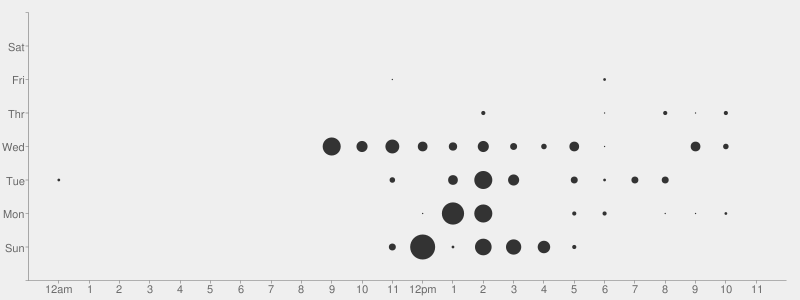
\includegraphics[width=\textwidth]{punchcard.png}
  \end{center}
  \caption{Punchcard som viser antall endringer på github vom funksjon av tid}
  \label{fig:punchcard}
\end{figure}
Fra denne figuren framgår det at onsdag og søndag hovedsaklig har vært gruppas
jobbedager, der gruppa har møttes og arbeidet sammen. I tillegg har det blitt satt
frister til onsdag for at ting skal være gjort, noe som reflekteres i at mye
arbeid har skjedd på mandag og tirsdag. Til sammenlikning er torsdag, fredag og
lørdag nesten uten arbeid.

\section{Beslutningsmønstre}
I gruppekontrakten (se \cref{avs:kontrakt}) står det at beslutninger fortrinnsvis
skal tas basert på konsensus, mens det ved splid skal være flertallsavgjørelse.
Gruppa var tidlig innstilt på konsensusavgjørelser, da det sørger for gode og
grundige diskusjoner ved uenighet, og kan i den forstand virke veldig samlende
for en gruppe. Likevel innså vi at enkelte situasjoner kunne bli fullstendig
fastlåst, slik at flertallet måtte få bestemme. Det er likevel viktig at
konsensus har blitt \emph{forsøkt} oppnådd før flertallsavgjørelse
implementeres. $\\$

Den første avgjørelsen gruppa tok var valg av oppgave. Åsmund var i starten
veldig giret på skiforsøket, som gikk ut på å måle spenstforfallet i en
slalomski utover sesongen. Resten av gruppa var noe mer moderate i
begeistringen. Det ble derfor arrangert ``høring'' hvor samtlige gruppemedlemmer
kom med forslag. Disse ble så samlet og diskutert, og gruppa forsøkte å finne en
oppgave hvor alle kunne bidra. Valget falt derfor på steking av bacon i
microbølgeovn, da dette hadde et massivt innslag av numerikk, programmering og
fysikk. Disipliner gruppa dekte meget godt mellom seg. $\\$

I samarbeidskontrakten er gruppestrukturen betegnet som ``riddere av det runde
bord''. Dette er et prinsipp som anvendes i alle våre beslutninger. Når et
problem oppstår går ordet rundt bordet, og hvert gruppemedlem sier sin mening.
Det diskuteres deretter i plenum, og om mulig oppnås en konsensusavgjørelse. Vi
har kun ved ett tilfelle anvendt flertall-paragrafen i kontrakten og det var i
forbindelse med språkvalg på prosessrapporten. Knut var i utgangspunktet uvillig
til å skrive på norsk, og det gikk ikke å ``vinne'' han over. Etter noen
minutter med diskusjon ble altså Knut Halvor overstyrt.

\section{Roller i gruppen}
"En person blir en leder når han eller hun blir satt i en lederposisjon."\\

I gruppekontrakten ble det bestemt at vi skulle ha en flatstruktur i gruppen. Valget 
var basert på at ingen egentlig ville gå inn i en lederrolle, og at vi ville ha en 
større frihet til å formulere arbeidsoppgavene selv. Vi kom likevel opp i situasjoner
som krevde at en person tok ledelse for å sikre effektiviteten til gruppen. I praksis 
fikk gruppen en situasjonsbetinget lederstruktur. Situsjonsbetinget lederskap er definert
som delt lederskap blant gruppemedlemmer der medlemmene varierer oppførselen etter hva
funksjon gruppen trenger til enhver tid, der en funksjon er en aksjon som blir satt 
igang for å sikre effektiviteten i gruppen.\\

Den situasjonsbetinget lederstrukturen førte og til at gruppemedlemmer tok rollen som 
leder i den fagdelen de hadde mest autoritet på. Åsmund ble dermed en uformell leder 
for fysikkdelen, Turid for numerikk delen og Knut for programmeringsdelen i C++. De 
tok dermed ansvar for fremgangen og oppgavedeling på disse områdene, og strukturerte 
samarbeidet mellom gruppemedlemmene på sitt respektive felt. \\

I vår gruppe såg vi at Åsmund i større grad gikk inn i rollen som oppgave-leder. Han 
tok ansvar for å sette opp et system for utveksling av informasjon rundt prosjektet, 
github, og tok ofte initiativ ved å legge ut relevante artikler på siden. Han gikk 
dermed og inn i rollen som koordinator (ref) på gruppen. Vi merket oss og at han var 
mer aktiv i prosjektet i EIT, som er den delen som er mest oppgavefokusert. \\

Bales statuerer at medlemmer som er veldig oppgavefokusert er mindre involvert i 
relasjonsrettet aksjoner. (ref) Paul er den i gruppen som er mest oppgavefokusert. 
På gruppa har han en tendens til å ta en faglig tilnærming, og liker å fokusere mest 
på oppgava for hånd. Han faller altså oftere inn i rollen som diagnostiker (ref) og 
informasjonssøkeren (ref). Han er dermed en styrke på gruppen ved at han holder 
diskusjonene relevante, i tillegg til at han er et pålitelig medlem når det gjelder 
å gjennomføre arbeidet i tide. Vi ser likevel en tendens til at Paul er mindre involvert 
i relasjonsrettet aksjoner på gruppa. \\

Den som oftest gikk inn i rollen som sosial-emosjonell leder var Turid. Hun var et viktig 
ledd i gruppen i form av å uttrykke klare meninger og frustrasjoner over moment i gruppen
som ikke fungerte optimalt. Hun gikk dermed inn i rollen som kritiker og følelsetolker (ref).
Når det var ting som fungerte bra i gruppen kom hun og inn med støtte og oppmuntring til å 
fortsette på samme linje. Selv om hun var en av de som oftest var involvert i diskusjoner/konflikter,
var hun og ofte den som løste de, enten gjennom forhandlinger eller ved å trekke seg tilbake
når hun gikk for langt. Turid var og det medlemmet i gruppen som oftest tok initiativ og ledelse 
i prosessdelen av EIT, som fokuserer mest på relasjoner og samarbeid mellom medlemmer på gruppen. 
Her virket hun ofte som målvakt (ref), ved å igangsette runde rundt bordet og være oppmerksom på 
at alle kom til ordet. Vi legger merke til at de situasjonene der Turid har
lederrollen i gruppa gjør at hennes rolle implisitt ligner mer på en tradisjonelle lederrolle, der de
andre har mer fagspesifikke lederroller. 
Situasjon: Paul og Turid.\\

Bale's statuerer og at sosial-emosjonelle aksjoner ofte blir igangsatt av medlemmer som er 
mindre involverte i oppgaveretta aksjoner. Dette ser vi igjen i gruppen ved at Joakim var 
involvert flere sosial-emosjonelle aksjoner. Denne situasjonen har oppstått ved at prosjektet 
er noe utenfor hans fagfelt, og han er dermed blitt mindre involvert i selve oppgaveløysingen. 
Joakim har delvis valgt dette bevisst ved en landsby der hans fagkompetanse ikke
står sterkest. Da hans rolle blir mindre faglig, kommer han naturlig inn i en
rolle som er mer i retning av en fasilitator for godt gruppemiljø. At ett av
gruppemedlemmene har hatt en slik rolle, i tillegg til å bidra faglig, har
utvilsomt gjort at gruppa har hatt høy ytelse når vi jobber, og heller tar
naturlige pauser med god stemning og humor nå medlemmene er slitne. Dette har
nok også hatt en effekt på at medlemmene i gruppa ble fort kjent med hverandre.
Joakim har utfylt denne rollen blant annet ved å alltid stille med en positiv innstilling og 
å involvere gruppen i diskusjoner som går på andre ting enn kun det faglige.\\

Det bor en liten kritiker i samtlige medlemmer på gruppen. Vi ser likevel at Knut har tatt på 
seg denne rollen i gruppen i større grad enn andre. Kritikeren er viktig i gruppesammenheng 
ved «systematisk, åpen, støttende og kritisk gransking av sitt og andres bidrag til gruppearbeidet.»
Dette gjøres på en slik måte at medlemmer på gruppa ikke opplever kritikken som en trussel, 
og dermed beholder fokuset på oppgaveløsning. (Innlegg frå andre).\\

\begin{figure}[ht!]
\centering
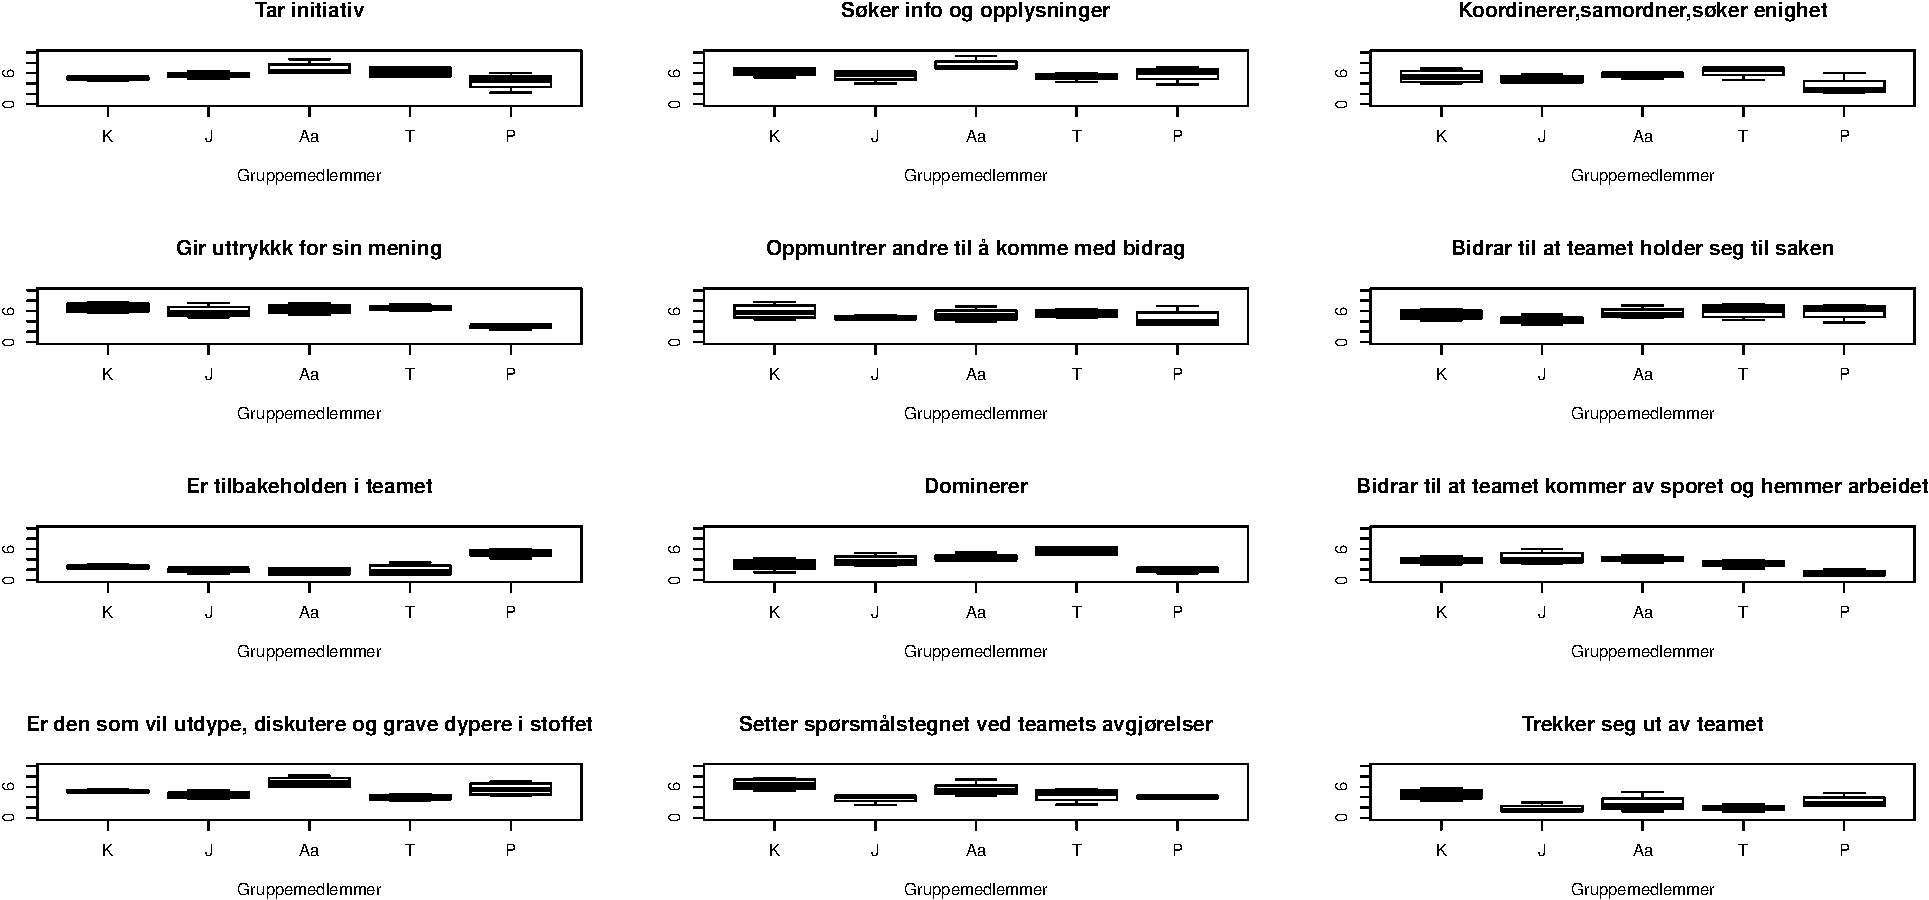
\includegraphics[scale=0.4]{teammedlem.pdf}
\caption{Plot av egenskaper til medlemmer på gruppen}
\label{fig:medlemmer}
\end{figure}

I \cref{fig:medlemmer} har vi brukt den ene prosessøvelsen til 
lage eit plot over egenskepene til gruppemedlemmene. Me ser at dei personlege egenskapene reflekteres 
igjen i dei rollene gruppemedlemmer har tatt på gruppen. Som gruppas kritikker ser me at Knut skårer 
høgt på punktet; setter spørsmålsteikn ved teamets avgjørelser. Han skårer og høgere på punktet; trekker
seg ut av teamet; som igjen kan trekkes tilbake til at han har ein lederposisjon ved implimentering av
programmet, som er noe sjølvstendig arbeid. Joakim skiller seg mest fra gruppen på punktet; Bidrar til at teamet 
sporer av. Det kan relateres tilbake til Joakims rolle som energigiver. Den beste måten å lade opp att
for videre jobbing av prosjekt er ofte ved å få litt avspredele frå sjølve oppgåvejobbinga.
Åsmund skårer høgt på punkta; tar initiativ og søker info og opplysninger. Dette kan relateres tilbake 
til lederrollen Åsmund har tatt for fysikkdelen avprosjektet som er veldig teoretisk. (Når ein prøver å 
modellere ein prosess realistisk kan modellen raskt bli komplisert. Det er da viktig  at me har nok 
informasjon til å kunne gjøre forenklinger som fremdeles resulterer i eit realistisk modell).
Turid er den som skårer høyset på punkta; dominerer og koordinerer, samordner, søker enighet, som igjen kan
relateres tilbake til den rollen hun har hatt som sosial-emosjonell leder. Ellers legg me merke til at gruppa
generelt er flinke til å ta initiativ, søkje info/opplysninger og gi uttrykk for sine meininger. Paul er den 
i teamet som er mest oppgåvefokusert, og me ser ein tendens i modellen til at han skårer noko høgare på 
tilbakeholden i teamet.

ref // (1) Handbok for gruppearbeidet\\
%bruk \cite{svenskeboka} - Åsmund

\section{Tilbakeblikk}
\label{sec:tilbakeblikk}

Når vi ser tilbake kan det påstås at gruppa gjennomgikk de fire trinnene i
Tuckmans \cite{tuckman} teori om gruppeutvikling, \emph{forming, storming,
norming} og \emph{performing}, selv om tildels har hoppet helt over
\emph{storming}-fasen. Dette har sin årsak i at vi er rimelig like i måten å
håndtere konflikter og at vi ikke kverulerer unødvendig, men er heller
løsningsorienterte og har fokus på fremdrift. At Tuckmans modell ikke passer
helt i dagens grupper (det er en gammel teori fra 1965), passer godt med Endre
Sjøvolds \cite{sjovold} påstander om at den er i ferd med å bli overflødig. Vi
kjenner oss også godt igjen i Sjøvolds evaluering av EiT-grupper, som basert på
Systematisere Person-Gruppe Relasjonen-modellen (SPGR) sier at utviklingen i en
EiT-gruppe ikke er signifikant (se \cref{tab:sjovold}).

\begin{table}[ht!]
\centering
\begin{tabular}{l c c}
& Pre & Post \\ \hline
Kontroll & 3.15 & 3.00 \\
Åpenhet & 4.71 & 4.61 \\
Avhengighet & 5.54 & 5.48 \\
Opposisjon & 1.50 & 1.36 \\
Innesluttethet & 1.20 & 1.09 \\
Synergi & 6.51 & 6.54 \\ \hline
\end{tabular}
\caption{Resultater fra Sjøvolds studie av EiT-grupper over ett semester, ser at
det ikke er noen signifikant forandring før/etter.}
\label{tab:sjovold}
\end{table}

Vi har likevel en kommentar til Sjøvolds konklusjon vedrørende kategorien
\emph{åpenhet}. Selv om gruppa nok er like åpen nå ved slutten enn ved oppstart,
er terskelen for å være åpen med andre gruppemedlemmer om problemer, kritikk
o.l., lavere. Slik at eksponeringen over tid har gjort interaksjonen mellom
medlemmene mer ukomplisert. Vi erkjenner likevel at rollene hver enkelt påtok
seg ved starten, har forblitt tilnærmet uforandret gjennom semesteret.
 %Tilsvarende den ``røde delen'' på prosessrapport-presentasjonen.
	%Overskrifter er kokt, endre dem så det passer.

%Kommentarene nedenfor gjelder situasjoner og elementer fra gruppelogg som skal
%dras inn. I tillegg må det reflekteres, og relevant teori må dras inn
\chapter{Analyse av gruppearbeidet}

\section{Kompetanse i praksis}

Samtlige gruppemedlemmer følger sivilingeniørstudiet på NTNU, og har som en
konsekvens av det den samme faglige ``grunnpakken''. Dette har gjort det enklere
for gruppemedlemmene og kommunisere på tvers av fagfeltene, da alle behersker
basisterminologi innen f.eks. fysikk, matematikk, statistikk og data. Utover
dette har gruppemedlemmenes kompetanse fått praktisk utfoldelse gjennom det vi
godt kan kalle naturlig oppgavefordeling. Knut Halvor, med bakgrunn fra
datateknikk, har hatt hovedansvar for programmering. Fysikeren på gruppa,
Åsmund, har taklet differensialligningenes praktiske anvendelse, mens gapet
mellom programimplementasjon og fysisk problem har blitt fylt (les:
diskretisert) av Turid og Paul, matematikerene på gruppa. Joakim, som har
spesialisering innenfor konstruksjonsteknikk, har bidratt litt over det hele, da
han har generell kunnskap innen de samme fagfeltene. Gjennom tilbakemelding på
gruppelogger viste det seg også at Joakim var flink til å skrive prosess, slik
at han fikk tildelt endel ansvar med tanke på prosessrapport. \\

Det har i så måte vært meget tilfredstillende og se at teoretisk kunnskap kan
benyttes til å beskrive praktiske fysiske fenomener, og at overenstemmelsen
mellom numerisk simulering og eksperiment er god. \\ 

\emph{Jeg fant dette kapittelet tungt å skrive om, vi må ha mer her.. Plenum
plz?!}

%Føler denne kan inn her - Åsmund
Som et eksempel på kompetanse i praksis presenterer vi en grafisk fremstilling
av et utdrag av loggen på github, \cref{fig:github}.
\begin{figure}[h!]
  \begin{center}
    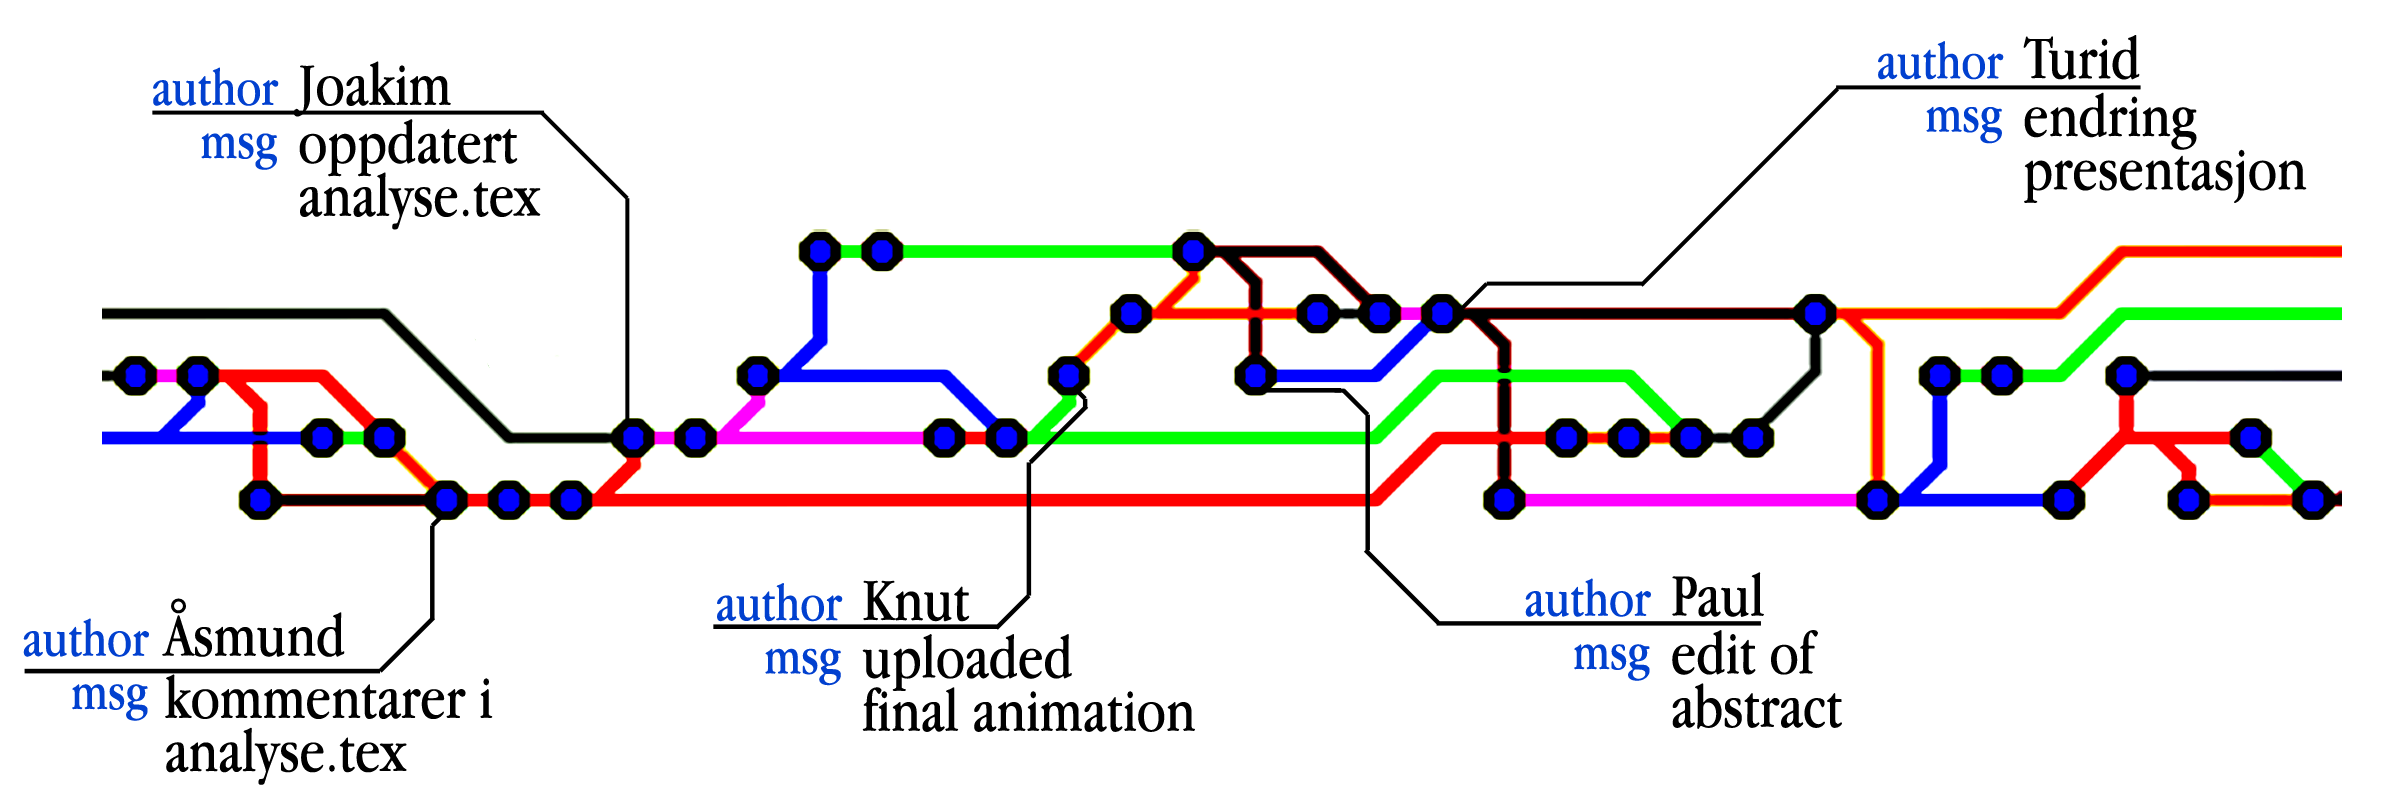
\includegraphics[width=1.1\textwidth]{github.png}
  \end{center}
  \caption{Et utdrag fra commit-treet for arbeidet på github}
  \label{fig:github}
\end{figure}
Her ser man hvordan de forskjellige medlemmene både har arbeidet på forskjellige
deler av prosjektet, og hvordan man har samarbeidet og gitt feedback på
hverandre: først har Joakim endret ``analyse.tex'', og så har Åsmund kommet med
kommentarer på den samme filen. Så har Knut lastet opp en fil som har med
numerikk-delen å gjøre, noe som er typisk for at han arbeider mer separat fra
resten. Så har Paul endret på rapporten, mens Turid har endret på
presentasjonen. Det fremgår også fra den kompliserte trestrukturen at alle
medlemmene bidrar på alle deler; i et team der alle bare jobbet med sitt ville
strukturen vært omtrent bare parallelle linjer.

\section{Kommunikasjon og samspill}
Det kommunikasjonsnettverket som ble brukt på gruppa vår var åpent nettverk og sirkel nettverk. 
I et åpent nettverk kommuniserer alle med alle. Denne formen for kommunikasjon kommer tydelig fram 
i diskusjoner på gruppen der det er fri flyt av ideer og meninger. Når en avgjørelse blir tatt på 
gruppen starter vi ofte med en åpen diskusjon, og utvekslinger av meninger. Før en avgjørelse blir 
tatt har vi vanligvis hatt en runde rundt bordet der alle får uttrykt sin mening om saken. Dette er 
en form for sirkel nettverk, der et medlem uttrykker sin mening før han sender ordet videre til sidemannen.
 Dette er en kommunikasjonsform som har utviklet seg naturlig på gruppen. Særlig i prosessdelen har 
 det falt naturlig å ta en runde rundt bordet for å høre de ulike medlemmenes meninger og følelser. 
 Her er det ofte Turid som har tatt initiativ til runde rundt bordet, og har dermed falt inn i en 
 rolle som ordstyrer. Etterhvert som gruppen ble bedre kjent var det flere som gikk inn i rollen 
 som ordstyrer, når de følte det var nødvendig. Dette førte til at vi fikk en naturlig styringsprosess
  ved gruppediskusjoner, uten at vi trengte å skrive en formell regel i gruppekontrakten.\\

%%%%%%%%%%%%%%%%%%%%%%%%%%%%%%%%%%%%%%%%%%%%%%%%%%%%%%%%%%%%%%%%%%
Gruppelogg 11:
Etter lunsj var det en meget god gruppeaktivitet i regi læringsassistentene.
Gruppemedlemmene skulle ved hjelp av poeng, rangere seg selv og gruppemedlemmer
i ulike situasjoner. Vi hadde på forhånd bestemt oss for at presentasjonen av
gruppa i prosessrapporten skulle inneholde to aspekter pr. gruppemedlem.
\begin{itemize}
\item Gruppemedlemmets egen oppfatning av seg selv
\item Gruppas oppfatning av personen
\end{itemize}
Altså var denne biten av prosessrapporten en naturlig forlengelse av øvingen, og
dermed noe vi følte vi hadde stort utbytte av.

Verdt å kommentere er at gruppen (tilsynelatende) virker meget trygge på hverandre.
Det var ingen pinlige og/eller flaue situasjoner i forbindelse med
poenggivningen, i tillegg til at vår selvoppfatning så ut til å passe godt med
gruppas oppfatning som helhet.\\

Det at egen selvoppfatning passer overens med gruppas oppfatning, viser at me har ein god
forståelse av uttrykksmåtene til dei andre medlemmene på gruppen. Dette viser at gruppemedlemmer
klarer å formidle hva de presenterer/står for på ein slik måte at andre sitter igjen med det samme bilde 
som gruppemedlemmet prøver å formidle. Dette viser tilbake til ein effektiv kommunikasjon på gruppen 
(\ref{sec:kommunikasjonsteori}).\\

Gruppelogg 4:
Det noteres at gruppedynamikken har blitt ganske god iløpet av disse ukene, og
debatten rundt problemstilling var frisk og nyansert. Diskusjonene fører til noe
konkret, og folk er flinke til å myldre og å bygge på andres ideer. Når gruppa
er enige om at nå skal vi gjøre noe, tar folk personlig initiativ uten at andre
pusher på.\\
%%%%%%%%%%%%%%%%%%%%%%%%%%%%%%%%%%%%%%%%%%%%%%%%%%%%%%%%%%%%%%%%%%
Det ble tidlig lagt normer som skulle gjelde for kommunikasjon i gruppen. I gruppekontrakten innførte vi kaffemøte om morgenen, 
for å diskutere framgangen og planlegge dagen videre. (Her åpnet vi og for at folk kunne ta opp ting før vi starta dagen.) 
Vi var likevel dårlig til å gjennomføre dette tiltaket i starten. Dette førte til at noen av medlemmene satt uten arbeidsoppgaver,
 og uten oversikt over hva de andre arbeidet med. \\

I gruppelogg dag 6 skriv gruppen;
På grunn av presentasjonen av faglitteratur, samt oppgavepresentering fra en gruppe,
idag tidlig, mistet vi vårt morgenmøte. Vi fikk derfor ikke tildelt arbeidsoppgaver på                                                         
en god måte, og starten ble litt ``flytende''. Turid og Paul satte igang med diskretisering
av sine differensialligninger, Åsmund jobbet med kurvetilpasning og Knut samarbeidet
med Turid og Paul om anvendelighet opp mot programmering. Joakim følte seg da litt
tilsidesatt fordi han ikke hadde fått tildelt noen spesifikk arbeidsoppgave. Det har derfor
blitt besluttet at arbeidsoppgaver skal avklares før noen setter i gang, slik at vi unngår at                                           
enkeltpersoner skal føle seg overflødig. Et positivt aspekt ved denne situasjonen var at
gruppetryggheten er så pass at Joakim kunne si hva han følte, og at gruppen da hjalp til
med å finne en relevant arbeidsoppgave. Etter denne hendelsen ble det dermed lagt større vekt 
på gjennomførelsen av kaffemøtet. Dette bedret effektiviteten til gruppen ved å sysselsette 
alle medlemmene og førte til at hvert medlem hadde en større oversikt over hva de andre arbeidet
med. I tillegg satt kaffemøte en offisiell start på dagen, og bidrog til et større samhold i gruppen. \\\

Andre tiltak?\\

Miljøet og fysiske faktorer kan ha en stor innvirkning på kommunikasjonen i
gruppen (\ref{sec:kommunikasjonsteori}). Vi har selv
merket at kommunikasjonen ofte blir skarpere og mer ampert når vi har jobbet over en lengre og
intensiv periode uten pauser. Dette har vi prøvd å gjort noe med ved å være flinkere til å ta
pauser. Spesielt når noen merker at andre medlemmer på gruppa begynner å bli slitne og irritable
er det viktig at andre tar initiativ til pauser. Rommet vi satt på hadde og dårlig ventilasjon,
noe som førte til at gruppemedlemmer fort ble tunge i hodet og slitne. I etterkant ser vi at
vi kunne vært mer selektive på lokale vi valgte å jobbe i, siden miljøet har mye å si for 
trivselen til medlemmene.(Hvordan gruppemedlemmer velger sittearrangementet, kan si mye om 
dynamikken i gruppen. Vi arrangerte bordet vi satt rundt som et kvadrat. Det var dermed ingen
plasser rundt bordet som gav en høyere status til noen av medlemmene, noe som understreker den 
flate strukturen på gruppen.)\\

En annen viktig faktor på gruppen som lettet kommunikasjonen på gruppen er bruk
av humor (\ref{sec:kommunikasjonsteori}). Dette er noe
som går igjen i gruppen vår. Helt frå begynnelsen har det vært en lett og god stemning mellom gruppemedlemmene. 
Dette gjør at vi har en lavere terskel for å uttrykke sterke meninger eller uenigheter. Vi har og en høy grad 
av selvironi på gruppen. Det at gruppemedlemmer ikke tar seg selv så høytidelige, gjør at det blir lettere å ta 
opp ikke-tema. Gjennom studier er det og vist at effektiviteten til gruppen øker ved bruk av passende og ofte 
selvrettet humor. Gjennom bruk av humor på gruppen, har vi blitt tryggere på hverandre, og dermed jobbet sammen 
mer effektivt. Vi er ikke redde for å tråkke hverandre på ``tærne'', noe som gjør at vi kan være den vi er. \\

Aksjoner for å betre gruppekommunikasjonen. Kaffepause, runde rundt bordet osv.!\\

\section{Situasjon gruppelogg 12}
Vi har hatt framføring av grupperapport og prosessrapport idag. Gruppen er fornøyd med egen innsats, da 
vi fekk sagt det vi skulle innenfor de rammene som var gitt. I en slik situasjon merker vi og at den 
tryggheten og innbyrdes tilliten vi har i gruppen er med å bidrar til en større trygghet i framføringen. 
Det at vi vet vi har tillit frå gruppen gjør at vi tør å improvisere mer i framføringen, noe som gjør 
framføringen mer levende. Vi merker og at de andre på gruppene følger med på hva en sier når en snakker, 
og er flinke til å hjelpe en videre dersom en setter seg fast på et ord eller setning. Dette virker som 
ei ``sikringsline'' som gjør at vi tør å gå litt utenfor våre respektive komfortsoner. Vi klarte og å beholde 
humoren vi har ellers i gruppen, noe som gir at spenningen blant de gruppemedlemmer som er ukomfortable 
med å stå foran en mengde blir lavere. ``Humor tends to promote cohesiveness and reduce tension in groups'' 
(Bloch, Browning \& McGrath 1983).\\
%Situasjon: øvelsen med evaluering ``det enkelte teammedlem''
%Situasjon: legomannen - bruk gruppelogg, men prøv å dra parallell til hvordan vi arbeider generelt.


\section{Bruk av regler/kontrakt}
%Situasjon: Knut Halvor og språk på prosessrapport

Gruppen ble tidlig enig om at prosjektrapporten skulle skrives på engelsk, så på
dette punktet oppnådde vi, i overenstemmelse med samarbeidskontrakten (appendiks
XXXXXX) - en konsensusavgjørelse. Da gruppa skulle avgjøre språket i
prosessrapporten ble det større problemer. Knut Halvor og Paul var veldig for å
skrive på engelsk, mens Turid, Joakim og Åsmund helst ville skrive på norsk. Det
ble, i henhold til J\&J \cite{jj}, Wheelan \cite{wheelan} óg Schwarz
\cite{schwarz} - arrangert en runde rundt bordet hvor hver enkelt måtte legge
frem argumenter for sitt standpunkt. Dette ble gjort for at uenigheten skulle
bli brukt til noe positivt, og at gruppa skulle komme mer sammensveist ut av
tvisten. Dette samsvarer godt med J\&Js teori (se \cref{sec:jj}) som beskriver
fire steg for effektivt å forbedre en gruppeidentitet: presenter egne meninger,
lytt til andres meninger, dann en felles gruppeidentitet - anta denne identiten.
På grunn av punktet om konsensusavgjørelser i samarbeidskontrakten, ble det
derfor brukt mye tid på å prøve og nå nettopp det. Etter godt og vel en time med
diskutering skjærte derfor Knut Halvor i gjennom og ba om en
flertallsavgjørelse. Dette er i henhold til gruppas beslutningsmønster, som sier
at ved manglende konsensus skal flertallet bestemme. Avstemmingen resulterte i
at prosessrapporten skulle skrives på bokmål. Paul skriver i sin private logg ``selv om jeg var uenig i at rapporten skulle
skrives på norsk, gjør prosessen rundt avgjørelsen det lettere å takle
`nederlaget' ''. Dette viser bare at Johnson \& Johnson sin teori \cite{jj} om
hvordan å få ulikheter blant gruppemedlemmene til å styrke gruppen fungerer i
praksis. \\

Dette illustrerer godt at gruppemedlemmenes personlige egenskaper er rimelig
like på et grunnleggende nivå. Ingen på gruppa er kverulerende i den forstand at
når de først har bestemt seg, så må det gjøres på hans/hennes måte. Overført til
denne situasjonen; selv om Knut \emph{egentlig} vil skrive på
engelsk innser han at det aldri vil nås konsensus og foreslår
flertallsavgjøring. På den måten sørger han for at effektiviteten ikke går ned
til null, men tvinger fremgang ut av en fastlåst situasjon. 

%Situasjon: Rapportering da Joakim var syk
Et annet eksempel på anvendelse av samarbeidskontrakten var da Joakim lå syk. I
gruppeloggen står det ``Joakim sendte SMS til gruppa før oppmøte, han handler
dermed i tråd med gruppekontrakten som sier; `gi beskjed dersom du ikke kan
møte'.'' Turid skriver i dagboka ``Det var greit å få beskjed om at Joakim var
syk på starten av dagen. På denne måten ble ikke gruppa unødvendig heftet i form
av å vente på siste person.'' Her ser vi godt at noe som kunne være årsaken til
en situasjon, blir avverget i form av klare regler/avtaler mellom
gruppemedlemmene. Og noe som potensielt kunne skadet gruppeånden (ved at Joakim
bare hadde holdt seg hjemme, for først å si fra senere på dagen), bidrar til å
styrke den. Med å styrke gruppeånden menes at de resterende gruppemedlemmene ser
at reglene brukes aktivt, og at Joakim tar hensyn og etterfølger disse. Dette
bidrar til økt tillit mellom gruppemedlemmene.


\section{Teori vs. virkelighet}
%Humor, selvironi, selvhøytidelighet - stemmer bra jamført teori
En teori vi lærte om veldig tidlig var Schwarz' grupperegler for effektivt
samarbeid (\cref{sec:schwarz}). Gruppa brukte tid på å sette seg inn i disse, slik at
hvert enkelt medlem skulle ha en felles forståelse av hvordan effektivt
gruppearbeid fungerte. Dette var lærdom som ble brukt titt og ofte, spesielt i
forbindelse med gruppelogger. Vi ble derfor overrasket da vi omtrent halvveis ut
i prosjektet så at medlemmene ikke hadde oversikt fremgangen, og at dette var et
direkte brudd på regel nummer 7: ``Utform fremgangsplan og tilbakemeldingsmåter
i plenum''. Mangelen på en fremdriftsplan hadde ført til at enkelte
gruppemedlemmer begynte å bli stresset, Turid skriver i sin private logg ``jeg
begynner å bli stresset, og er redd for at vi ikke skal bli ferdig i tide''.
$\\$

Neste landsbydag luftet Turid frustrasjonen under kaffemøtet. Det viste seg at
Joakim, Paul og Knut følte det på samme måte, mens Åsmund hadde rimelig god
oversikt. Dette hadde sin naturlige årsak i at Åsmund tidlig hadde påtatt seg
rollen som layout-ansvarlig, og at alt nytt materiale gikk til han. Det ble
derfor meget tydelig at målt fremdrift måtte formaliseres, slik at hver enkelt
kunne få tilgang til nåværende status. Det ble derfort gjennomført en revisjon
av samarbeidskontrakten (se \cref{sec:kontrakt}), i form av et punkt om oppføring av
status og fremdriftsplan fra gang til gang. Vi erfarer her at
tilbakemeldingssystemet innad i gruppa fungerer, selv om det tok litt lang tid
før problemet ble oppdaget. I tillegg ser vi at gruppereglene til Scharwz
(\cref{tab:grunnregler}) har noe for seg, og at å droppe kun én faktisk
resulterer i lavere effektivitet. \\


%Situasjon: ``In your face!'' fra Turid til Joakim om Crank og stabilitet
Ved oppstart ble det tidlig diskutert hvilket diskretiseringsskjema som skulle
brukes på differensiallignignene. Da diskusjonen peilet seg inn på
Crank-Nicolson-skjemaet påpekte Turid at dette var ubetinga stabilt for varmelikningen. Dette
sa Joakim seg uenig i, da han mente å huske noe om ustabilitet i forbindelse med
nevnte skjema. Argumentene utviklet seg etterhvert til å bli rimelig usaklige, i
form av Turids ``jo, den er stabil'' mot Joakims ``nei, den er ustabil'', man
kan vel også legge til at stemningen bygget seg noe opp. Det endte med at Åsmund
sjekket ut Crank-Nicolson-skjemaet på wikipedia, hvor det i en av de første
setningene stod: ``spesielt kan nevnes at Crank-Nicolson-skjemaet er
\emph{ubetinget} stabilt''. I seiersrus avsluttet Turid diskusjonen med å sende
avgårde en ``ìn your face'' til Joakim. $\\$

 Det ble likevelt sagt med et smil om munnen, noe også Joakim oppfattet. 
Og det hele gruppa lo av situasjonen i ettertid. Knut skriver i sin personlige
logg ``Vi hadde en potensiell situasjon idag mellom Turid og Joakim. Heldigvis
såg alle parter humoren i utsagnet. Det virker som det er god humor blant gruppemedlemmene''.

Likevel kan man i etter-på-klokskapens lys se potensielle faremomenter
i hendelsen. Joakim kunne tatt seg nær av det Turid sa, og valgt å holde sine
meninger for seg selv fremover i frykt for å bli latterliggjort igjen. Men, i
egenskap av gruppens medlemmer ikke tar seg selv så høytidelig ble dette en
situasjon som bidro til at vi ble bedre kjent. Vi så at det er/var
rimelig stor takhøyde for hva som kunne bli sagt, noe som utvilsomt har påvirket
kommunikasjonen i ettertid. Dette har ført til at kritikk lettere
har kommet frem, og at hvert gruppemedlem heller ikke har vært redd for å motta
den. Man kan godt si at gruppemedlemmens sammenfallende humoristiske sans har
gjort grensene og tersklene for å ta opp ``ubehagelige'' ting lavere, da ein klarer å 
sjå eventuelt humor i situasjonen. Med ein uhøytidlig atmosfære på gruppen vet gruppemedlemmer
og at eventuell kritikk ikke blir tatt for personleg. Vi observerer altså her at teorien 
som tar for seg humor (\cite{jj-humor} og \cref{sec:kommunikasjonsteori}) stemmer 
meget godt med humors innvirkning på gruppeprosesser i virkeligheten.
    %tilsvarende den brune delen
	\chapter{Konklusjon}
Allerede på de første landsbydagene la vi merke til at vi hadde hatt flaks med
gruppesammensetningen. Alle gruppas medlemmer var innstilte på å gjøre en god
jobb, og vi merket fort at stemningen i gruppa var god. På starten var vi
noe negativt innstilt til jobbing med prosess. Vi så ikke på forhånd nytten
av å dedikere spesifikk tid til å arbeide med teambygging, og mente at teambygging
ville skje naturlig dersom vi bare fikk jobbe med prosjektet. \\

Etterhvert som vi fikk jobbet noen ganger med prosjekt og med prosess så vi at
prosessarbeidet har en klar nytteverdi. Øvelsene har i seg selv vært ganske
gode, selv om det har vært litt murring, hovedsaklig fordi det har avbrutt oss
mens vi var godt igang med prosjektarbeidet. Det at vi har arbeidet med prosess
samt å tilegne oss teori har ført til at grupperegler har ligget i bakhodet når
situasjoner har oppstått, slik at vi har tatt teorien i bruk i praksis, f.eks.
når vi .\\

Vi har også merket at vår tilegnelse av teorien har gjort det enklere å håndtere
situasjoner som har med gruppestruktur og gruppedynamikk å gjøre. Når man kan henvise
til en bestemt teori som underbygger argumenter for å omstrukturere er det
enklere å bli enige om et felles ståsted.\\

Den største endringen i gruppedynamikken så vi under framføringen i midten av
semesteret. Medlemmene fikk inntrykk av at de andre på gruppa var oppmerksomme
når man snakket, og at man fikk god støtte hvis man ble utrygg. Dette gjorde at
flere av medlemmene følte seg trygge nok til å improvisere med eksempler rundt
gruppas framgang. \\



%Appendikser:
	\appendix
\chapter{Program source code}
\label{ap:source_code}
\section{Main file}

\lstinputlisting[language=C++]{../program/source/main.cpp}

\section{Physical constants header file}

\lstinputlisting[language=C++]{../program/source/headers/phys_consts.h}

\section{Physical constants implementation}

\lstinputlisting[language=C++]{../program/source/phys_consts.cpp}

\section{Physical system header file}

\lstinputlisting[language=C++]{../program/source/headers/phys_sys.h}

\section{Physical system implementation}

\lstinputlisting[language=C++]{../program/source/phys_sys.cpp}

\section{Conjugate gradient method header file}

\lstinputlisting[language=C++]{../program/source/headers/cgsolver.h}

\section{Conjugate gradient mehtod implementation}

\lstinputlisting[language=C++]{../program/source/cgsolver.cpp}

\section{Script to plot raw data from program using gnuplot}

\lstinputlisting[language=bash]{../program/build/plot.sh}

\section{Script to make movie of plots using ffmpeg}

\lstinputlisting[language=bash]{../program/build/animate.sh}

\section{Makefile}

\lstinputlisting[language=make]{../program/build/Makefile}





	
%Referanser
	\bibliographystyle{plain}
	\bibliography{referanser.bib}
	\coffee{1}
\end{document}

